\section{Aufbau und Durchführung}
\label{sec:Durchführung}
\subsection{Aufbau}

\begin{figure}[H]
  \centering
  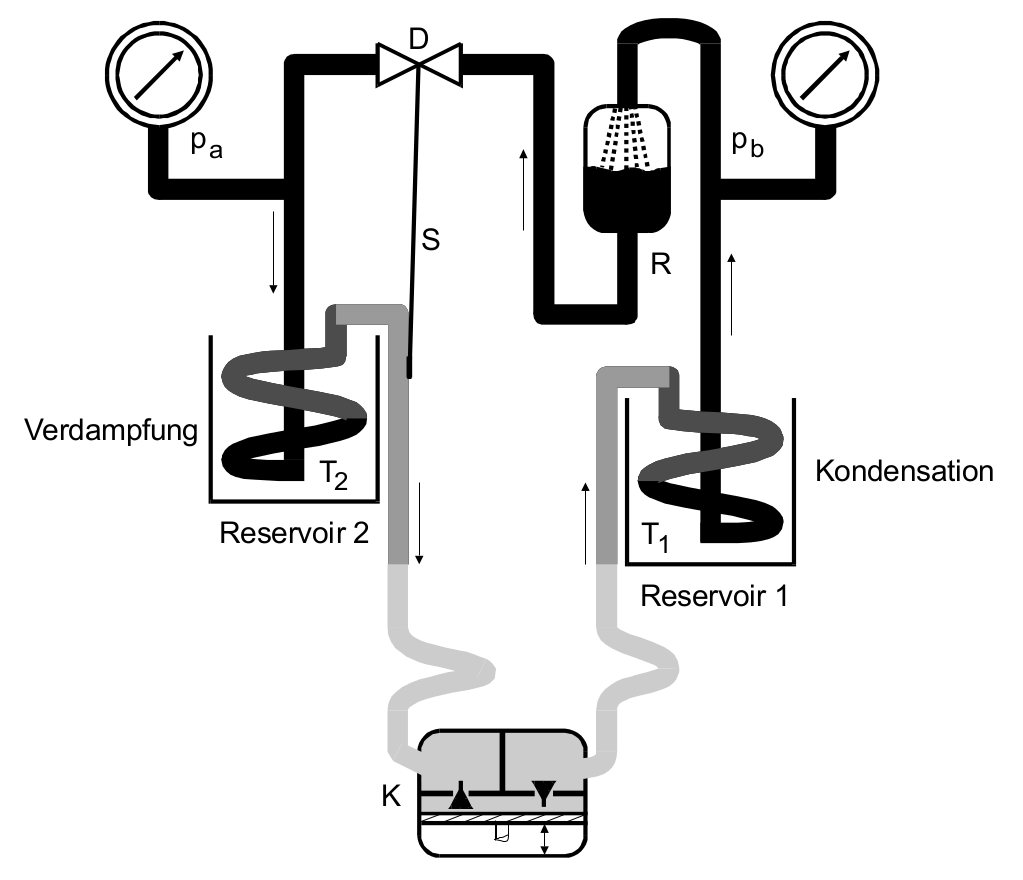
\includegraphics[height=6cm]{skizze.png}
  \caption{Skizze der Wärmepumpe.}
  \label{fig:skizze}
\end{figure}

Das Grundgerüst der Wärmepumpe bildet ein Kupferrohr, welches ein Transportmedium beinhaltet.
Dieses Medium kann Wärmeenergie in Form von Phasenumwandlungsenergie aufnehmen bzw. abgeben.
Es empfiehlt sich, einen Stoff mit möglichst hoher Kondensationswärme zu verwenden, um einen möglichst effizienten Wärmetransport zu ermöglichen.
Deshalb wird beim vorliegenden Aufbau Dichlordifluormethan ($\ce{Cl2F2C}$) eingesetzt.\\
Vom Kompressor K, welcher den Mediumkreislauf ermöglicht, durchläuft es das erste Reservoir $R_1$.
Unser reales Gas wurde nun so gewählt, dass es in $R_1$ bei der Temperatur $T_1$ sowie dem Druck $p_b$ flüssig wird.
Jenes Medium gibt beim Phasenübergang von gasförmig zu flüssig die Kondensationswärme ab, die es im Reservoir $R_2$ als Verdampfungswärme $L$ pro Gramm aufgenommen hat.
Daraufhin durchläuft die Flüssigkeit ein Drosselventil.
Der Strömungswiderstand am Drosselventil sorgt für den nötigen Druckunterschied $p_b-p_a$.
Hinter dem Druckventil durchläuft das Medium das Reservoir $R_2$.
Durch den hier vorherschenden Druck $p_a$ und die Temperatur $T_2$ verdampft die Flüssigkeit und nimmt die latente Wärme $L$ auf.
Wieder im Kompressor angekommen wird das Gas nahezu adiabatisch komprimiert.
Der Druck steigt erneut an, so dass sich das Medium wieder verflüssigt und der Kreislauf fortgesetzt wird.\\
Zusätzlich befindet sich zwischen dem Reservoir $R_1$ und dem Drosselventil $D$ ein Reiniger $C$, welcher die Flüssigkeit von Gasrückständen befreit.
Gleichzeitig bewahrt das Drosselventil $D$ den Kompressor davor, dass Flüssigkeitsreste in ihn gelangen.
Beide Elemente sind jedoch nur aus Sicherheitsgründen installiert, so dass eine problemlose Durchführung gewährleistet ist.
Sie spielen physikalisch für das Ergebnis keine Rolle.\\
Die beiden Rührmotoren gewährleisten eine gleichmäßige Temperaturverteilung im jeweiligen Reservoir.\\
Die interessanten Größen in diesem Versuch sind die Temperaturen $T_1$ und $T_2$, die Drücke $p_b$ und $p_a$ sowie die Kompressorleistung $P$.

\subsection{Durchführung}
Vor Versuchsbeginn wurden die beiden Reservoire mit genau abgemessenen $\SI{4}{\litre}$ Wasser befüllt.
Danach wurden sie möglichst isoliert an den vorgegebenen Kupferspiralen positioniert.
Unmittelbar nach dem Einschalten der Rührmotoren und des Kompressors wurden ab Minute 0 im Abstand von einer Minute die Temperaturen $T_1$ und $T_2$ an den jeweiligen Thermometern, sowie die beiden Drücke $ p_b $ und $ p_a $ an den jeweiligen Manometern und die Kompressorleistung $ P_K $ am Wattmeter gemessen und tabellarisch notiert.\\
Die Temperaturen wurden auf 0,1 $ \si{\celsius} $ genau gemessen.
Die Druckskala von $ p_b $ konnte man auf $ \SI{0,1}{\bar} $ ablesen, die von $ p_a $ auf $ \SI{0,2}{\bar} $.
Die Kompressorleistung wurde auf $ \SI{1}{\watt} $ genau bestimmt.\\
Der Versuch endete nach dem Erreichen von $ \SI{50}{\celsius} $ in $ R_1 $ (nach $ \SI{30}{\minute} $).
Anschließend wurden noch den beiden Manometern die Drucktemperaturen zum Erstellen einer Dampfdruckkurve entnommen.
\label{sec:Durchführung}
